
\chapter{Statistical Models}  
\label{chap:mixed}  

Let $Y_{ij}$ denote the rating user $i$ gives item $j$.   As before,
most of these values are unknown, and thus we wish to predict them.
That latter point suggests regression modeling, which we will do in this
chapter.  We'll use both the classical linear and logistic models, as
well as machine learning methods.

\section{Latent Factor Models} 

The most basic model here is

\begin{equation}
Y_{ij} = \mu + \alpha_i + \beta_j + \epsilon_{ij},~ i = 1,...,m;~ j =
1,...,N_{i.}
\end{equation}

where $m$ is the number of users and $N_{i.}$ is the number of ratings
we have for user $i$.  (Define $N_{.j}$ to be the number of users rating
item $j$.) Other than $\mu$, all terms have expected value 0.  The terms
are interpreted as follows:

\begin{itemize}

\item $\mu$:  overall mean rating of all items, past, present and future

\item $\mu + \alpha_i$: overall mean rating of all items, past, present
and future, by user $i$; $\alpha_i$ then reflects a tendency for user
$i$ to give more liberal ratings ($\alpha_i >0$) or harsher ratings
($\alpha_i < 0$)

\item $\mu + \beta_j$: overall mean rating of item $j$ by all users,
past, present and future; $\beta_j$ then reflects a tendency for item
$j$ to receive more liberal ratings ($\beta_j >0$) or harsher ratings
($\beta_j < 0$)

\item $\epsilon_{ij}$ is a ``miscellaneous'' term that account for
all factors not accounted for in the model

\end{itemize} 

The $\alpha_i$ and $\beta_j$ terms are called \textit{latent} factors, a
term meaning ``hidden.''  We can't observe user, say, 29's tendency to give
high or low ratings; it's just a model for some kind of driving force in
that user's behavior.  The ``synthetic, representative'' users in
Chapter \ref{chap:svd} are also called \textit{latent} in the RS
literature.

The analogous model for logistic regression, i.e.\ binary $Y$, is

\begin{equation}
P(Y_{ij} = 1 ~|~ i,j) = 
\frac{1}{1 + \exp[-(\mu + \alpha_i + \beta_j)]}
\end{equation}

\subsection{Estimating the Latent Factors}

To predict the unobserved $Y_{ij}$, we will need to estimate $\mu$ and
the $\alpha_i$ and $\beta_j$.  Let's see how.

\subsubsection{Linear Case}

Intuitively, estimators in the linear case are simply sample analogs of
the corresponding population quantities:

\begin{equation}
Y_{..} = \widehat{\mu} = \frac{1}{N} \sum_{i,j \textrm{ obs.}} Y_{ij}
\end{equation}

\begin{equation}
\label{yi.}
Y_{i.} = \widehat{\mu} + \widehat{\alpha}_i = \frac{1}{N_{i.}}
\sum_{j, \textrm{ obs.}} Y_{ij}
\end{equation}

\begin{equation}
\label{y.j}
Y_{.j} = \widehat{\mu} + \widehat{\beta}_j = \frac{1}{N_{.j}}
\sum_{i, \textrm{ obs.}} Y_{ij}
\end{equation}

where $N = \sum_{i} N_{i.}$ and ``obs.'' means summation over all
observed values, i.e.\ not the missing ones.  So 

\begin{equation}
\widehat{\alpha}_i = Y_{i.}-Y_{..},~ 
\widehat{\beta}_j = Y_{.j}-Y_{..}
% \frac{1}{N_{i.}} 
% \sum_{j, \textrm{ obs.}}^{N_{i.}} Y_{ij}
% - \frac{1}{N} \sum_{i,j \textrm{ obs.}} Y_{ij}
\end{equation}

The reader may recognize the latter two quantities as the biases from
the preceding chapter (without $Y_{..}$).

\subsubsection{Logistic Case}

The approach of the last section, a special case of a technique called
the \textit{Method of Moments}, would not work as well in the logistic
case.  For example, consider (\ref{yi.}), which would now be, for each
$i$,

\begin{equation}
\label{nonlin1}
\widehat{\mu} + \widehat{\alpha}_i = 
\frac{1}{N_{i.}} \sum_{j=1, \textrm{ obs.}}
\frac{1}{1 + \exp[-(\widehat{\mu} + \widehat{\alpha_i} + \widehat{\beta_j})]}
\end{equation}

We have a similar set of equations (as $j$ varies) corresponding to
items.  We'd now have a set of nonlinear equations to solve.

Instead, what people use is the \textit{Method of Maximum Likelihood}.
To be sure, we still have a set of nonlinear equations to solve, but MLE
has certain optimal statistical properties, and the \textbf{lme4}
package (included in \textbf{rectools}) uses MLE, so we'll go that
route.\footnote{The \textbf{mle} package is for a general class of
methods known as \textit{mixed models}, not specifically for RS.}

To see how MLE works, consider the following game.  I toss a coin until
I accumulate $r$ heads.  I don't tell you what value I've chosen for
$r$, but I do tell you $K$, the number of tosses I needed.  You then
must guess the value of $r$.  Well, elementary probability calculations 
show that\footnote{This is a family of distributions known as
\textit{negative binomial.}}

\begin{equation}
\label{negbin}
P(K = u) = \binom{u-1}{r-1} 0.5^u,~ u = r, r+1, ...
\end{equation}

Say I tell you $K = 7$.  Then what you might do is find the value of $r$
that maximizes 

\begin{equation}
\label{negbin7}
\binom{6}{r-1} 0.5^5
\end{equation}

You are asking, ``What value of $r$ would have made our data ($K = 7$)
most likely?''  Trying $r = 1,2,...,5$, one finds that $r = 4$ maximizes
(\ref{negbin7}), so we would take that as our guess.\footnote{By the
way, here is how the Method of Moments approach would work here. For the
negative binomial distribution it is known that $E(K) = r/p$, where $p$
is the probability of ``success,'' in this setting meaning heads.  So
$E(K) = 2r$.  Under MM, we would set $\overline{K} = 2 \widehat{r}$,
where the left-hand side is the average of all values of $K$ in our
data.  We only did the ``experiment'' once, so $\overline{K} = 6$ and we
guess $r$ to be 3.5.  Of course, $r$ must be an integer, so we'd guess 3
o 4.}

Now back to the RS estimation.  It is assumed that the $\alpha_i$ and
$\beta_j$ are independent, normally distributed random variables.  The
joint likelihood of all the observed $Y_{ij}$ (now incorporating both
probabilities and probability density function values) is then quite
complex, but it can be maximized, which is what \textbf{lme4} does for
\textbf{rectools}.  

\subsection{Incorporation of Covariate Data}

Instead of the old model, 

\begin{equation}
Y = \mu + \alpha + \beta + \epsilon
\end{equation}

we now have

\begin{equation}
\label{modelwithcovs}
Y = X' \gamma + \alpha + \beta + \epsilon
\end{equation}

where $X$ is the vector of covariates and $\gamma$ is the vector of
linear regression coefficients.  Note that the old $\mu$ term is now
absent, at least explicitly.  It now has become $\gamma_0$, and $X$ has
a 1 component.  So for instance $X$ may be (1,age,gender).

\subsection{Estimation Approach}

Write the data version of the model (\ref{modelwithcovs}), with
estimates rather than population values, as 

\begin{equation}
Y_{ij} = X_{ij}' \widehat{\gamma} +
\widehat{\alpha}_i + \widehat{\beta_j} + \widehat{\epsilon}_{ij}
\end{equation}

Now, holding $i$ fixed, average both sides over $j$.  The left side will
be $Y_{i.}$.  Since $E\beta = E\epsilon = 0$ and we assume independence,
the average of the last two terms will be about 0.  So, the average of
the right side will be approximately

\begin{equation}
\overline{X}_{i.}' \widehat{\gamma} +
\widehat{\alpha}_{i} 
\end{equation}

where the vector $\overline{X}_{i.}$ is the average value of the vectors
$X_{ij}$ over $j$.

Setting this to (\ref{yi.}), we have

\begin{equation}
\widehat{\alpha}_i = 
Y_{i.} -
\overline{X}_{i.}' \widehat{\gamma} 
\end{equation}

Similarly,

\begin{equation}
\widehat{\beta}_j = 
Y_{.j} -
\overline{X}_{i.}' \widehat{\gamma} 
\end{equation}

\subsection{Example:  InstEval Data}

\begin{lstlisting}
> getInstEval()
> mmout <- trainMM(ivl)
\end{lstlisting}

Let's browse:

\begin{lstlisting}
> names(mmout)
[1] "alphai" "betaj"  "lmout"  "Ni."    "N.j" 
> mmout$alphai[4]
     1000 
-1.095866 
> mmout$alphai[5]
    1001 
0.892603 
\end{lstlisting}

So user 1000 seems to give harsher ratings than average, while user 1001
is more liberal in her ratings.\footnote{The reader may wonder why user
1000 would show up fourth in this vector of $\widehat{\alpha}_i$.  The
reason is that the code indexes users by the character form of their
IDs.}

The above used the covariates.  Here is the no-covariates version:

\begin{lstlisting}
mmout.nocov <- trainMM(ivl[,1:3])
\end{lstlisting}

Let's predict the rating user 8 would give instructor 72:\footnote{As an
exercise, the reader should check that our observed data does not
contain this rating, but that instructor 72 is in the data.}

\begin{lstlisting}
> predict(mmout.nocov,matrix(c(8,72),nrow=1))
[1] 2.912437
\end{lstlisting}

\subsection{Implementation}

Below are excerpts of the code from \textbf{trainMM()}.  First, we find
(\ref{yi.}) and (\ref{y.j}):

\begin{lstlisting}
haveCovs <- ncol(ratingsIn) > 3
n <- nrow(ratingsIn)
userRowGrps <- split(1:n, users)
itemRowGrps <- split(1:n, items)
uimean <- function(uirowgrp) mean(ratings[uirowgrp])
Yi. <- sapply(userRowGrps, uimean)
Y.j <- sapply(itemRowGrps, uimean)
\end{lstlisting}

Now for the covariates case:

\begin{lstlisting}
cmd <- paste("lmout <- lm(", nms[3], " ~ .,data=ratingsIn[,-(1:2)])",
    sep = "")
eval(parse(text = cmd))
xmeans <- function(uirowgrp) colMeans(ratingsIn[uirowgrp,
    -(1:3), drop = FALSE])
Xi. <- t(sapply(userRowGrps, xmeans))
X.j <- t(sapply(itemRowGrps, xmeans))
predsa <- predict(lmout, as.data.frame(Xi.))
predsb <- predict(lmout, as.data.frame(X.j))
...
alphai <- Yi. - predsa
betaj <- Y.j - predsb
\end{lstlisting}

Since we want to make use of the original variable names, we built up
the \textbf{lm()} call as a character string, then execute that string.

\section{Full Regression Models}

As will be seen shortly, it is natural to consider regression models for
the $Y_{ij}$.  To illustrate this, let's again consider the InstEval
data.

\subsection{Linear, Logistic}
\label{linlog}

In the original form of the InstEval data, i.e.\ not the one returned
from the \textbf{rectools} function \textbf{getInstEval()}, the first
two columns, which are the user and item IDs, are R factors.  Assuming
for now that we are not using covariates, we could
then make a call like

\begin{lstlisting}
lm(y ~ s + d, data=InstEval[,c(1,2,7]) 
\end{lstlisting}

Recall that R automatically converts factor predictors to dummy
variables, in this case 2972 of them for user IDs and 1128 for item IDs.
We could then use the return value in \textbf{predict()} calls.
The case of binary $Y$ and a logistic model would be handled similarly.
If we do use covariates, simply specify \textbf{data=InstEval} above.

This will lead to long run times, since we will have so many predictors,
in this case 2972+1128 = 4100 of them.  Indeed, that is why \textbf{lme4}
has a long run time.

However, the use of dummies in the linear case is essentially the same
as our Method of Moments approach earlier in this chapter.  This
suggests a better way:  Take our $Yi.$ and $Y.j$
as our new data.

For instance, here is row 51 of InstEval (for compactness,
without covariates):

\begin{lstlisting}
   s    d y 
51 8 1884 5       
\end{lstlisting}

The value of (\ref{yi.}) for user 8 is

\begin{lstlisting}
> tapply(InstEval$y,InstEval$s,mean)['8']
  8 
3.8 
\end{lstlisting}

while (\ref{y.j}) is

\begin{lstlisting}
> tapply(InstEval$y,InstEval$d,mean)['1884']
    1884 
3.141176 
\end{lstlisting}

We could then replace row 51 by

\begin{lstlisting}
   s    d    y 
51 3.8  3.14 5       
\end{lstlisting}

We then call \textbf{lm()} on the new data.  Let's call this the
``$\alpha,\beta$ Regression Method.''

The \textbf{rectools} function \textbf{RStoReg()} performs this
transformation, including covariates, if any.

\subsection{Creating New Covariates}

In the InstEval data, suppose some instructors do especially well in
service courses.  How might we take this into account?

In the parametric case, say \textbf{lm()} or \textbf{glm()},
the naive way would be to include interaction terms corresponding to
combinations of the \textbf{d} and \textbf{service} columns in the data
frame.  This would mean products of the dummy variables for item ID and
the dummy for service course.  But as noted in Section \ref{linlog}, we
are already at risk of overfitting, and probably can ill afford adding
many terms of this type.

\subsubsection{Dimension Reduction}

An alternative would be as follows.  In our transformed data (output of
\textbf{RStoReg()}), in addition to the columns corresponding to
estimated $\alpha$ and $\beta$, we could have a column for mean rating
in service courses.  Again consider row 51 in the data, originally

\begin{lstlisting}
   s    d y 
51 8 1884 5       
\end{lstlisting}

and transformed to

\begin{lstlisting}
   s    d    y 
51 3.8  3.14 5       
\end{lstlisting}

Now suppose instructor 1884 has an average of 4.8 in service courses.
Our new row 51 would be

\begin{lstlisting}
   s    d    v   y 
51 3.8  3.14 4.8 5       
\end{lstlisting}

If we then perform an analysis using \textbf{lm()} we are adding only
one element to the ``$\beta$'' vector -- much better than adding 1128
parameters, one for each of the products of the dummies for the
instructors and the service dummy.

Of course, various other applications of this trick would be possible.
For example, often there are students who do very well in one department
but less well in others.

One problem, though, say in the service course example, would be that
some instructors never teach service courses, and thus there would be no
value for them in the \textbf{v} column above.  One solution would be to
do subsetting:  We would divide our raw data into two sets, one for
instructors who teach service courses and the other for the rest.  We
could fit the richer model on the first subset, while not including this
aspect in the second.

\subsubsection{Polynomial Mdels}

As in Section \ref{prgengex}, we can create new variables by adding
polynomial terms to a linear or logistic model.

Why are polynomials helpful?  First, the regression function may not be
linear in the predictors.  For instance, the relation of wage income to
age tends to be nonmonotonic, rising until about age 40, then falling
somewhat.

Second, keep in mind that polynomials include cross-product terms.
Say $U$ and $V$ are dummy variables.  Then a polynomial in them of
degree 2 or higher will include not only terms like $U^2 = U$ and $V$,
but also $UV$.

Say for example in the InstEval data service courses in department 5
have an average student rating of over 4.00.  Take $U$ and $V$ to be
dummies for department 5 and high service course rating.  Then $UV$ is
an indicator for the situation in which the course is a service course
in department 5, and we would like a variable ($UV$) that flags this
condition.

Since there are only a few departments, this approach would not run
afoul of the overfitting concerns described earlier, where our 118
instructors would give rise to 1128 new variables.

\subsection{Machine Learning}

Though typically presented in terms worthy of science fiction --- the
name \textit{machine learning} itself sounding SciFi-ish --- the fact is
that machine learning(ML) techniques are simply methods for estimating
regression functions (including, recall, the case of binary response,
i.e. classification).  They are nonparametic, like kNN, and thus differ
from, say, linear and logistic models, but in the end, they are just
regression estimators.

Hee we will discuss the ML method that generally gets the most
attention, neural networks (NNs).  Various other techniques are also
ppular, such \textit{random forests}, \textit{boosting} and
\textit{Support Vector Machines}.\footnote{Technically, our treatment
here will cover just \textit{feedforward} NNs.  Another type
\textit{convolutional} NNs, is popular in image classification
applications.  These really are not any different from basic NNs; the
``C'' part consists of standard image-processing operations that long
predate NNs and are widely used in non-NN contexts.  \textit{Recurrent}
NNs, popular for text classication, allow loop connections but otherwise
have standard NN structure.}

\subsubsection{Example: Predicting Vertebral Abnormalities}

Here six predictors are used to guess one of three vertebral conditions,
normal (NO), disk hernia (DH) and spondylolisthesis (SL).  The picture
below was generated by the R package \textbf{neuralnet}.

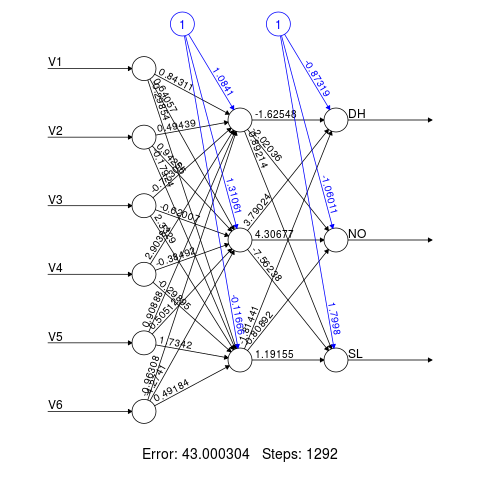
\includegraphics[width=5.6in]{Images/VertebraeNN.png} 

There are three \textit{layers} here, vertical columns of circles.  
The flow is from left to right.\footnote{As mentioned, in an RNN there
would also be loops.}  The values of the six predictors for a particular
patient, \textbf{V1} through \textbf{V6} enter on the left, and our
predicted class for that patient comes out of the rightmost layer.
(Actually, the three outputs are class probabilities, and our predicted
class will be taken to be the one with highest probability.)

The circles are called \textit{neurons} or simply \textit{units}.  At
each unit, a linear combination of the inputs is computed as an output.
The outputs of one layer are fed into the next layer as inputs, but only
after being run through an \textit{activation function},
say\footnote{This of course is the function used in logistic regression,
but there really is no connection.  In each case, one needs an
increasing function with values in (0,1), conditions that this function
satisfies.}

\begin{equation}
\label{logit}
a(t) = \frac{1}{1 + e^{-t}}
\end{equation}

The activation function is applied to the outputs of the circles. The
activation function can be different in each layer.

To make things concrete, look at that middle layer, specifically the top
unit.  There are six inputs, corresponding to the six predictors
variables.  Each input has a \textit{weight}.  \textbf{V1}, for
instance, has the weight 0,84311.

This at first sounds like the action of \textbf{lm()}, but the key
difference is that we are computing three different sets of weights, one
for each of the three units in that middle layer.  The weight of
\textbf{V1} into the second unit is 0.64057.  To allow for a constant
term like in linear regression models, there are also ``1'' inputs, seen
at the top of the figure.  The outputs of the second layer also get
weights, for input into the third layer.

The number of layers, and the number of units per layer, are
hyperparameters, chosen by the analyst.

So, how are the weights determined?  It's an iterative process (note the
word ``steps'' in the caption of the figure), in which we are trying to
optimize some loss function, e.g.\ mean squared prediction error.  The
process can become quite complex, and in fact much of NN technology is
devoted to making the iteration process faster and more accurate.  We
will not pursue that here, other than to note that many of the
hyperparameters in any NN implementation are devoted to improving in
those senses.

\subsubsection{But What Is \emph{Really} Going On?}

With all this complexity, it is easy to miss how NNs work.  To gain
insight, consider an activation function $a(t) = t^2$.  This is not a
common one at all, but let's start with it.

As noted, the inputs to the second layer are linear combinations of the
first layer values.  But due to the activation function, the outputs of
that second layer will be squared, so that the inputs of the third layer
are --- read carefully --- linear combinations of \textit{squares} of
linear combinations of \textbf{V1} through \textbf{V6}.  That means
quadratic polynomials in \textbf{V1} through \textbf{V6}.  If we were to
have several more hidden layers, then the next layer would output
polynomials of degree 4, then degree 8 and so on.

What about other activation functins $a(t)$?  For any polynomial $a(t)$,
you can see again that we will have polynomials of higher and higher
degree as we go from layer to layer.

And what about (\ref{logit})?  Recall from calculus that one can
approximate a function like that with a Taylor series --- i.e.\ a
polynomial!  And even some common activation functions like one called
\textit{reLU} that lack Taylor series can still be approximated by
polynomials.

In other words:

\begin{quote}
\textbf{Key point:}  NNs are really just polynomial regression.
\end{quote}

But you can see this can cause serious problems of overfitting.  We saw
in the example in Section \ref{prgengex} that things really got out of
hand, even with degree 7.  The polynomial degree that can be tolerated
will depend on the size of dataset, but clearly we have a major issue
here.

In other words:

\begin{quote}
\textbf{Key point:}  NNs are highly prone to overfitting.
\end{quote}

So, how do NN advocates deal with this?  The answer is that they have an
array of techniques to ameliorate overfitting.  One method is
\textit{dropout}, in which some units are randomly culled from the
network, thus achieving dimension reduction.  Another method involves
\textit{regularization}, which as we have seen earlier consists of
shrinking the weights.

As usual, the typical tool for hyperparameter selection is
cross-validation, but with so many hyperparameters, we do need to worry
about p-hacking.

\subsubsection{R Packages}

There are many R packages available for NNs.  At present, the most
sophisticated is \textbf{Keras}, an R implementation of a popular
general algorithm of the same name.  The \textbf{kerasformula} package,
acting as a wrapper to \textbf{keras}, gives the user a more ``R-like''
interface.\footnote{For installation tips, see
\url{https://keras.rstudio.com}.}

Let's look at the code we'll use in the next section:

\begin{lstlisting}
units <- c(5,2,NA)
layers <- list(units=units,activation=c('relu','relu','linear')) 
kfout <- kms(y ~ .,data=udconv[-idxs,],layers=layers) 
prd <- predict(kfout,udconv[idxs,-19]) 
preds <- 1 + 4 * prd$fit
\end{lstlisting}

In the first line, we are specifying layers consisting of 5 and 2 units,
followed by a layer that simply passes through output from the previous
layers.  In the second line, we are also specifying activation
functions, reLU for the first two layers, with 'linear' again meaning
passing data straight through.  This is because we have a regression
application here.  For a classification problem, we would probably
specify 'softmax' for our last activation functionn, which outputs the
index of the largest input.

The third and fourth lines are straightforward, typical R operations,
but the fifth requies explanation.  It is recommended that
typically one should \textit{center and scale} one's data, as this has
been found to help convergence properties.\footnote{One common issue is
the ``broken clock problem'' in which the algorithm converges but all
the predicted values are identical!}  One might, for instance, apply R's
\textbf{scale()} function to the predictor data, subtracting the means
and divided by the standrd deviations.

One might scale the response variable too.  In \textbf{kerasformula},
that variable is scaled down to [0,1], by subtracting the lower bound
and dividing by the range.  In the InstEval data, for example, since the
ratings range from 1 to 5, we subtract 1 and dividde by 5 - 1 = 4.
Since the predicted values come back on this same scale, we must
mulitply by 4 and add 1 in order to return to the original scale.


\section{Example: InstEval}

Let's try these methods on the InstEval data, and compare them to matrix
factorization:

\begin{lstlisting}
getInstEval()
set.seed(9999)
idxs <- sample(1:nrow(ivl),5000)
trn <- ivl[-idxs,]
tst <- ivl[idxs,]
# matrix factorization
mfout <- trainReco(trn)
preds.mf <- predict(mfout,tst[,-3])
mean(abs(preds.mf - tst[,3]),na.rm=T)  
# Method of Moments
mmout <- trainMM(trn)
preds.mm <- predict(mmout,tst[,-3])  
mean(abs(preds.mm - tst[,3]),na.rm=T)
# predict from alpha_i, beta_j, linear model
udconv <- RStoReg(ivl)
udconvout1 <- lm(y ~ .,data=udconv[-idxs,])
preds.conv1 <- predict(udconvout1,udconv[idxs,])
mean(abs(preds.conv1 - tst[,3]),na.rm=T)  
# predict from alpha_i, beta_j, linear model, deg. 2
library(polyreg)
pfout <- polyFit(udconv[-idxs,],2) 
preds <- predict(pfout,udconv[idxs,-19]) 
mean(abs(preds - udconv[idxs,19])) 
# predict from alpha_i, beta_j, NN
library(kerasformula)
units <- c(5,2,NA)
layers <- list(units=units,activation=c('relu','relu','linear')) 
kfout <- kms(y ~ .,data=udconv[-idxs,],layers=layers) 
prd <- predict(kfout,udconv[idxs,-19]) 
preds <- 1 + 4 * prd$fit
mean(abs(preds - udconv[idxs,19]))
\end{lstlisting}

\begin{table}
\begin{center}
\vskip 0.5in
\begin{tabular}{|r|r|}
\hline
method & MAPE \\ \hline 
\hline
MF & 1.038 \\ \hline 
MM & 1.012 \\ \hline 
$\alpha, \beta ~ \textrm{lin.}$ & 0.956 \\ \hline 
$\alpha, \beta ~ \textrm{poly.}$ & 0.954 \\ \hline 
$\alpha, \beta ~ \textrm{NN}$ & 0.959 \\ \hline 
\end{tabular}
\end{center}
\caption{}
\label{}
\end{table}

The $\alpha, \beta \textrm{ Regression}$ methods seemed to have a slight
edge.  But of course, the usual caveats:

\begin{itemize}

\item What works well on the InstEval data may not be so good, indeed
might be very poor, on some other data set.

\item We should do several runs of each experiment, averaging their
results or taking their median, to remove the sampling variation caused
by the random split.

\item We only tried the default rank in MF, and presented only an
NN configuration (two hidden layers, 5 and 2 neurons) which we found to work well.

\end{itemize} 
